\documentclass[conference]{IEEEtran}
%Template version as of 6/27/2024

\usepackage{cite}
\usepackage{amsmath,amssymb,amsfonts}
\usepackage{algorithmic}
\usepackage{graphicx}
\usepackage{textcomp}
\usepackage{xcolor}
\def\BibTeX{{\rm B\kern-.05em{\sc i\kern-.025em b}\kern-.08em
    T\kern-.1667em\lower.7ex\hbox{E}\kern-.125emX}}

\begin{document}

\title{Measuring the Effect of Context Perturbations on the Reliability of AI Agent Systems}

\author{Natalie Lambert}

\maketitle

\begin{abstract}
Artificial intelligence agent systems driven by Large Language Models (LLMs) 
have evolved from simple zero-shot prompting into complex single-agent and multi-agent workflows
capable of multi-step problem solving, with minimal human intervention.
With agents solving longer, more difficult tasks, it becomes imperative to understand how context
management techniques and heuristics can be used for more reliable systems.
AI agent systems increasingly rely on orchestration techniques and execution constraints
to successfully complete tasks in a more consistent way.
This proposal presents an series experiments to 
observe how context perturbations, such as irrelevant information, context truncation
and context segment reordering, can impact reliability metrics for
single-agent and multi-agent systems when solving programming-related tasks.
Such an empirical study will be able to pinpoint the real problems in agent system reliability, as
well as place an upper bound on the expected variation of agent outputs for complex multi-step tasks.
\end{abstract}

\begin{IEEEkeywords}
artificial intelligence, multi-agent, single-agent, orchestration, benchmark, context, reliability.
\end{IEEEkeywords}

\section{Introduction}\label{intro}
AI agent systems is a branch of artificial intelligence research that examines how
models can be harnessed to exhibit emergent reasoning and step-by-step problem-solving, given a
specific input task definition.
These systems are said to have \emph{agency} if there is little to no human involvement while the
system plans and executes the task at hand.
Although it is possible to harness any kinds of models in this way, the most prominent real-world
example is the application of AI agent systems that use Large Language Models (LLMs),
where a user inputs a natural language description of a task (called a user input prompt), and receives the
final result once the agent system has executed to completion.

Agentic architecture are ways in which LLMs and auxiliary tools can be organized, in order to allow
for a structured definition of how LLMs can interact with inputs and the surrounding environment.
Organizing and restricting how an LLM is allowed to process information and complete tasks acts as a
way to secure the system, so that the LLM cannot execute arbitrary steps that may be destructive.
Architectural decisions involve deciding how many of which kind of model are part of the system, how
resources are allocated between models, and which tools (e.g. for writing code, accessing local
files or browsing the Internet) are available.

Agent orchestration refers to the control layer that manages aspects such as task delegation,
data sharing, system state management and inter-agent communication.
In tandem with the structural definitions of the system architecture, orchestration implements the
actual processes that make an agentic system functional.
This constraint-focused perspective of AI agents has emerged from a trend towards the use of
so-called \emph{hybrid} systems, which borrow concepts and merge implementations of classical symbolic
AI frameworks and generative neural systems \cite{ali_agentic_2025}.
Since generative AI are inherently probabilistic in nature, they pose challenges in terms of
reproducibility and interpretability.
On the other hand, symbolic AI systems are rule-based, and are thus too inflexible to new workloads.
A common approach in designing agentic systems has been to incorporate aspects of both types of AI
systems, to provide an advantageous middle-ground in terms of adaptability and reliability.

With agentic system evaluation centred on accuracy and task completion scores, researchers have
shown that reliability metrics are just as important for comprehensive agent evaluations
\cite{rabanser_towards_2026}.
Researchers look to agent orchestration
techniques as a promising approach for improving task solving reliability, which allows for agent
harness designs that are LLM-agnostic.
The design principles that determine how an agentic system can be improved remain underexplored,
causing real-world deployments to rely heavily on incomplete empirical heuristics and ad hoc decisions
rather than principled, robust design and implementation \cite{kim_towards_2026}. 
Understanding these systems is foundational for solving tasks that require
sustained multi-step interactions, iterative information gathering under partial observability,
and adaptive strategy refinement.

This research will focus on quantifying the reliability degradation of Large Language Models (LLMs)
when context perturbations are injected during long-horizon task execution.
By injecting irrelevant data, pruning context proactively, and changing the ordering of context
segments, the aim is to identify the specific failure patterns triggered by context mismanagement
in both single-agent loops and a centralized multi-agent system with an orchestrator and sub-agents.

\section{Related Work}
Agentic systems have much in common with distributed systems, in that architectures are often composed 
of modular building blocks that have a clear interface for passing prompts, LLM responses and tool outputs. 
Understanding how an agentic system works hinges on examining the interaction of its modules,
and reasoning about how each individual component impacts the overall system.

Two categories of agentic architectures have emerged and are widely adopted.

\subsection{Single-Agent Systems}
A single-agent system is composed of a single LLM, surrounded by a minimal harness which allows for
tool-calling capabilities and iteration.
Despite the use of enhancements such as Retrieval Augmented Generation (RAG)
and the Model Context Protocol (MCP) \cite{ehtesham_survey_2025}, Single-Agent Systems (SAS) are not able
to solve tasks that are beyond a certain complexity,
since the context window of the central LLM is constrained \cite{gao_single-agent_2025, patel_dynamic_2026}.
While defining these tasks and categorizing the complexity is an open issue yet
to be fully addressed or quantified by an agentic benchmark, Single Agent Systems (SAS) 
are primarily used in the context of sequential tasks where maintaining a linear chain of thought 
is necessary \cite{kim_towards_2026}.

Furthermore, single agents struggle with data-intensive reasoning. 
In evaluations like LiveAgentBench, which tests agents against real-world web challenges across domains such 
as humanities, law, and economics, the best agents' accuracy score was 35\% compared to a 70\% human baseline, 
although the use of tool calls provided a 56\% boost over isolated LLMs \cite{li_liveagentbench_2026}. 
Moreover, a agent shows a tendency towards context drift (which leads to unhelpful hallucinations),
infinite loops, or a premature halt without completing the assigned task.

\subsection{Multi-Agent Systems}
A Multi-Agent System (MAS) is composed of two or more single agents that interact, which results in
a system that can decompose and parallelize tasks.
The literature identifies several structural organizations and collaboration strategies 
for MAS, ranging from pure cooperation to adversarial debate and competition
\cite{yarmohammadtoosky_llm-powered_2026, taleb_expansion-contraction_2026}.

Current MAS architectures face severe coordination complexities and scalability issues 
\cite{yarmohammadtoosky_llm-powered_2026, sampath_adaptive_nodate}. 
One of the most pronounced problems is topology-dependent error amplification. 
In completely independent multi-agent systems, unchecked error propagation results in up to 17x 
more errors than a single-agent baseline \cite{kim_towards_2026}. 
Even when a centralized \emph{orchestrator} agent (synonymous with central manager agent) 
is introduced to check errors, the error rate is still 4x that of the baseline, 
and the system suffers from a validation bottleneck at the orchestrator
\cite{kim_towards_2026, zhang_agentorchestra_2026}.
Moreover, the existence of a central leader agent node leads to a performance bottleneck, since
all sub-agents must wait for the leader agent to arbitrate and resolve inconsistencies in sub-task
completion.
To mitigate logical inconsistency, duplicate operations, and unbounded autonomy, 
robust coordination layers are strictly required \cite{adimulam_orchestration_2026, ruan_aorchestra_2026},
but a key challenge with MAS is the difficult task of transmitting the right amount of context 
between agents: papers discuss the existence of a phenomenon called context fragmentation.

While MAS have shown promise in handling more complex task resolutions, the continued (although
slow) improvements in frontier LLMs cause the gap to narrow between SAS and MAS accuracy scores
\cite{gao_single-agent_2025}.
Thus, MAS are not a panacea: they exhibit \emph{capability saturation},
which means that if a single-agent's base accuracy on a task exceeds 45\%, 
assigning multiple agents to the same task will generally incur higher coordination 
and compute costs than benefit gained from the increased accuracy score \cite{kim_towards_2026}.

\subsection{Context Management}
A recent survey on context engineering formalize this domain into a set of distinct, but
inter-related problems; 
specifically context evolution, information selection, context formatting and context fragmentation
remain key challenges \cite{mei_context_survey_2025}.
Although context management has been studied more frequently against foundation models,
it remains a central concern and under-explored topic for agentic system design.

Despite the increase in how much context can be handled by frontier models, recent research reveals
that using the maximum context window size without discerning the importance of information passed
to the LLM leads to unexpected effects and trade-offs.
For example, a phenomenon called the \emph{reasoning shift} occurs when a prompt is
padded with irrelevant context, shrinking the effective context by up to 65\% \cite{rodionov_reasoning_2026}.
The useless context triggers lazy behavior behaviour on the part of the LLM, which decreases the
amount of overall tokens spent on chain-of-thought reasoning and self-checking,
ultimately degrading accuracy on complex tasks.
This finding correlates with agentic systems inexplicably terminating early after
accumulating redundant and irrelevant context through many loop iterations over time.

Futhermore, experiments have demonstrated a drawback to extended context windows, termed
the \emph{lost in the middle} phenomenon, which demonstrates that decoder-only models struggle
to retrieve information when the key text is sandwiched 
in the middle of a long context window (2-6K tokens),
exhibiting worse accuracy scores than closed-book baselines \cite{liu_lost_nodate}.
Accuracy scores are highest only when crucial details are placed at the very beginning or end of the
context, similar to how humans are able to recall information due to recency or primacy bias.

While supervised fine-tuning can help models ignore noises \cite{rodionov_reasoning_2026},
and repeating queries can assist with synthetic key-value retrieval tasks \cite{liu_lost_nodate},
managing extraneous information remains a critical bottleneck for both standalone LLMs and composite
agentic systems that accumulate context for long-running tasks.
For centralized agentic systems, the orchestrator experience context bottlenecks more severely,
since they are often overwhelmed with large amounts of output from sub-agents \cite{patel_dynamic_2026}.

To counter problems with uncontrolled context growth, some agent systems adopt
database-inspired transactional safeguards and context pruning to prevent degradation due to poor context
management and to subsequently ensure state consistency.
\begin{itemize}
\item Transactional Integrity: SagaLLM implements mechanisms for consistency, 
	rollback, and the preservation of invariants as mechanisms for tracking context globally
	across agents \cite{chang_sagallm_2025}. 
	Since LLMs suffer from unreliable self-validation, SagaLLM uses an external
	LLM-as-judge to validate all agent outputs,
	with selective retention to actively filter out fluff \cite{chang_sagallm_2025}.
\item Semantic-Aware Context Repos: DynTaskMAS utilizes a hierarchical storage forest combined 
	with a 2-phase commit protocol. 
	These strategies allow multiple parallel agents to atomically update the global context repository 
	while semantic analysis guarantees that agents only retrieve the specific chunks 
	of context that they need \cite{yu_dyntaskmas_2025}.
\item Dynamic Attentional Context Scoping (DACS): Designed to resolve context competition among
	sub-agents within an orchestrator LLM, DACS implements a registry mode alongside agent-triggered
	focus sessions \cite{patel_dynamic_2026}. 
	By dynamically loading a single active agent's full context while offloading the remaining
	agents' context, DACS 30\% to 50\% increase in task steering accuracy with sublinear context scaling.
\end{itemize}
Although agentic systems attempt to address corner cases where context degradation is the
direct root cause of failures, most papers acknowledge that effective context management must not
come at the cost of a significant increase in overhead.

\subsection{Agent System Reliability}
Agent scalability and reliability have been identified as key issues in the literature
\cite{kim_towards_2026, rabanser_towards_2026}.

Despite continuous improvements in benchmark accuracy scores, 
AI agents frequently fail in real-world deployments, revealing a critical discrepancy 
between standard evaluations and actual in-practice use-cases. 
Current evaluation practices rely heavily on mean task success rates, omitting to 
capture what kinds of tasks fail, the severity of those failures, or how resilient an 
agent is to various input and environmental perturbations. 
To address this gap, a paper proposes drawing inspiration from safety-critical engineering to 
assess whether AI agents can ensure bounded errors, calling for a holistic
evaluation framework of concrete metrics across four key dimensions: 
consistency, robustness, predictability and safety \cite{rabanser_towards_2026}.

The consistency dimension is meant to evaluate repeatable behavior across multiple runs and includes 
metrics such as: 
\begin{itemize}
	\item Outcome: per-task success rate normalized against Bernoulli variance.
	\item Trajectory: measuring the distribution of agent action types used to complete a task and
		the Levenshtein distance across action sequences to track reasoning paths. 
	\item Resource Usage: determine the variation in important resource metrics, such as tokens,
		cost and GPU time, as well as how the resource usage varies across different runs.
\end{itemize}

The robustness dimension assesses agent stability by measuring the effect of fault-injected runs,
environmental perturbations, and semantically equivalent prompt variations. 
This phenomenon of token-level sensitivity is a known vulnerability where models overfit to specific 
token sequences rather than generalizing across semantic concepts, 
though reinforcement learning from human feedback (RLHF) can act as a partial mitigation
\cite{cox_mapping_2025}.

To address uncertainty, the predictability dimension assesses how well the agent system itself can identify
low-confidence responses \cite{rabanser_towards_2026}. Although it is a possible approach for
discerning possibly stable agent results, in practice LLMs are notoriously difficult to calibrate
and are not amenable to reliable self-introspection.

Finally, the safety dimension separates failure probability from failure consequences by evaluating 
compliance using an LLM-as-judge for identifying constraint violations, 
and assessing overall harm by computing aggregate severity scores. 
Even though these new metrics are collected when running agents against old benchmarks
like GAIA and $\tau$-bench \cite{mialon_gaia_2023, yao_tau-bench_2024},
findings indicate that while agent reliability shows a slight upward trend, 
it lags significantly behind raw accuracy scores \cite{rabanser_towards_2026}.

Traditional benchmarks frequently overlook operational realities, which makes it difficult to make
comprehensive evaluations.
Due to the increasing number of agentic system deployments, there has been a recent shift
towards balancing agent success rates with operational metrics such as cost and latency.
with operational metrics like cost, latency, and reliability
\cite{ding_hybrid_2024, mehta_beyond_2025, smirnova_cost-aware_2026}. 

\section{Methodology}
The key focus of the project is to determine how context perturbations contribute
to unreliable behaviour in the overall multi-agent system.
For an agentic system, the information in the context window evolves as the agent iterates over
multiple steps to reach a final output.
It is therefore useful to classify the different types of information that may be present in the
context window throughout the agent's execution time.
\begin{itemize}
	\item The \emph{initial user prompt} provides the requirements for the current task. The initial
		prompt outlines what the agentic system must solve, and what is expected for the final result.
	\item Chunks of information from a \emph{knowledge base} may be used to supplement the
		task-specific context from external sources. The agent is required to autonomously fetch and
		evaluate the relevance of this additional information.
	\item \emph{Tool invocations and outputs} act as stateful information of what action an agent
		has taken from a pool of available plug-ins in its environment,
		as well as the results from calling the tool.
\end{itemize}
During the resolution of a task, an agent may delete, truncate, overwrite, or otherwise modify any
of the above context information, usually due to context window size constraints.
Observed primacy and recency bias effects also provide a challenge; it is often ineffective
to include irrelevant context, which can hinder LLM reasoning, or lead to surprising inaccuracy due
to information reorganization within the context window \cite{liu_lost_nodate}.
Although some of these challenges have been studied for stand-alone LLMs, the full extent of these
effects on agent system reliability is unclear, especially in the situation where multi-agent
systems must cohesively manage context sharing between sub-agents.

\subsection{Research Questions}
For sophisticated tasks that require multiple steps and tool calls for completion,
it is advantageous to study how perturbations
(i.e. modifications to the context during the execution of a task)
can answer the following open questions.
\begin{enumerate}
	\item Does pruning irrelevant or outdated agent output from the context
		(e.g. error messages from running a unit test on a patch) deter significant deviations in
		expected agent behaviour?
	\item What is a heuristic that can be used to help discern which kind of irrelevant context 
		starts hurting agent reliability?
	\item To what extent does reordering of context during a task affect the reproducibiity of an
		agent's output?
	\item Is there a visible break-down in a multi-agent system that can be directly linked to
		poorly manage context and irrelevant context propagation?
	\item Is there a strategy that can be used to create clear management policies for
		different categories of context?
\end{enumerate}

\subsection{Experiment Design}
To obtain a baseline, it is necessary to test a series of context perturbation scenarios on a single
agent system, which operates in a simple ReAct (i.e. reasoning and acting) loop \cite{react_2023}.
The core aim is to examine context management for a single LLM whose harness provides minimalistic
functionality to call tools and iterate sequentially over the multiple steps required for a task.
As shown in Figure~\ref{fig-single-setup}, context evolves over time, which allows for context
modification during different iterations of a ReAct loop.

\begin{figure}[htbp]
\centerline{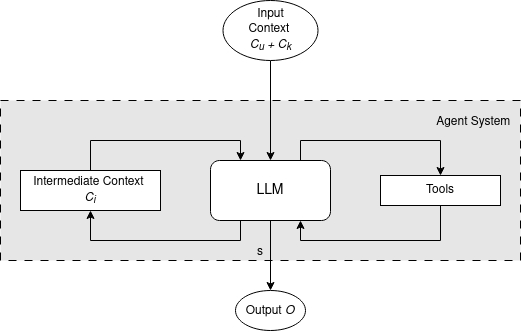
\includegraphics[width=2.5in]{../figures/sas-context.png}}
\caption{A schematic showing context evolution in a single-agent ReAct loop. After inputting the
	user's prompt $C_u$, concatenated with the knowledge base information $C_k$, the LLM in the
	agent harness iteratively calls tools and generates output ($C_i$ for each iteration $i$), until
	the execution terminates, and the agent outputs the final user-readable output $O$.}
\label{fig-single-setup}
\end{figure}

The subsequent milestone of the project will be to extend the same experiments to a centralized
multi-agent system, where an orchestrator manages sub-agents that contribute to the overall task.
Since the multi-agent version of the experiments will essentially examine the interaction between
agents as a medium for context mismanagement, it is necessary to focus on tracing to identify when
context perturbation in one sub-agent leads to final output instability for the entire system as a whole.
Figure~\ref{fig-multi-setup} provides a visualization for the injection of a perturbation in one
sub-agent, potentially leading to a significantly variation in the final output.

To test both the single-agent and multi-agent paradigms, this project will use the OpenHands agent
\cite{openhands_2026}, which is open source and supports both agentic architectures.
For accessibility, ease of deployment and transparency in the experimental set-up, the project will
involve open weights LLMs, such as GPT-OSS, Qwen3, Llama3 and Gemma3.
The proposed work is independent of the exact LLM version and model used, since the main goal is to
expose gaps in context management that can be addressed by the agentic harness.

\begin{figure}[htbp]
\centerline{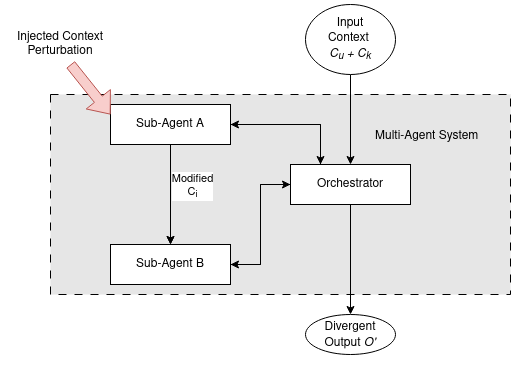
\includegraphics[width=2.5in]{../figures/mas-context.png}}
\caption{A diagram showing the tracing of a context perturbation across messages between sub-agents
	in a centralized multi-agent system. Each agent (including the orchestrator), is essentially the
	building block shown in Figure~\ref{fig-single-setup}, except for the addition of messages that
	can pass $C_m$ (i.e. relevant chunks of context) between agents.}
\label{fig-multi-setup}
\end{figure}

For a given context string $C_i$ during the execution of a task,
the following types of perturbations will be applied:
\begin{enumerate}
	\item Concatenate up to $N$ irrelevant chunks of information. For different trials, concatenate
		the irrelevant context at different locations in the context window.
	\item Prune $M$ chunks of context to see if proactive shortening of the context window leads to results.
		Like in the previous perturbation strategy, test pruning at different indices of the context window.
	\item Without removing or adding context chunks,
		simply reorder context segments to examine the importance of information ordering.
\end{enumerate}

For completeness, it will be necessary to test the above perturbation cases at various steps in the
completion of a task, including the input user prompt $C_u$, the intermediate task context $C_i$ for
different $i \in [1, \text{num\_tasks}]$, as well as knowledge base context $C_k$.

\subsection{Benchmark}
To ensure consistent comparisons of the outputs between different trials, this project is confined
to examining the coding benchmark, SWE Bench Pro \cite{swebenchpro_2025}.
SWE-Bench Pro builds off SWE-Bench \cite{jimenez_swe-bench_2024}, by providing more complex and long-horizon 
programming and bugfix tasks, which makes it appropriate for multi-agent task decomposition.
SWE-Bench Pro evaluates agents on how well they can resolve GitHub issues.
An agent completes a task successfuly based on how many unit tests pass in the repository when
including the generated code or bugfix.

Some recent benchmarks, such as GAIA2, rely on the use of a LLM-as-judge
to verify consistency, causality, timing, and completeness via rubrics rather than strict string matching. 
However, this approach is not fool-proof, and the lack of bounds on the LLM-as-judge's accuracy
poses unnecessary challenges in terms of reproducibility and statistical analysis \cite{froger_gaia2_2026}.
However, the benchmark introduced additional strict constraints on how runs were evaluated,
such as considering a benchmark run a failure
if it is forcefully terminated due to a timeout threshold or a context overflow; these are experimental
checks that are included in the Agent Research Environment (ARE) framework.
Thus, ARE will be used to set-up the benchmark runs and experiments,
because it provides customizable scaffolding for running benchmarks in a
controlled environment with agent monitoring capabilities \cite{froger_are_2025,froger_gaia2_2026}.

\subsection{Metrics}
In order to quantify how perturbations in context can affect the reliability of agentic systems,
it is necessary to focus on statistical measures that evaluate the probability of the agent's output
being reproducible and relatively free of noise.
Prior work has shown that agentic systems evaluations tend to focus on so-called
``performance'', i.e. accuracy scores, or what fraction of runs for a given task is awarded a ``pass''
(which depends highly on what a benchmark is trying to evaluate).
This project reuses some of the reliability metrics proposed in prior work, which makes a case
for examining agent reliability from a statistically sound perspective \cite{rabanser_towards_2026}.

It is assumed that there are $T$ tasks in the benchmark, each of which is run a total of $K$ times,
in order to average across measured quantities.
Each task can terminate in a binary outcome (i.e. pass or fail), so $y_{t,k}$ is defined as the
outcome $y$ for the $t$th task and $k$th run.

The project will measure the following quantities:
\begin{enumerate}
	\item \emph{Outcome consistency}: measures the extent to which the agent system is able to output
		the same result across many runs of the same task. Ideally, an agent can solve a task in a
		reproducible way, so this value (which has a range in $[0,1]$) should be as close to
		$1$ as possible. The formula for the metric is thus
		$$R_{con} = \frac{1}{T} \sum_{t=1}^T (2\hat{p}_t-1)^2$$
		where $\hat{p} = \frac{1}{K} \sum_{k=1}^K y_{t,k}$.\\
	\item \emph{Sequential trajectory}: for any given attempt at solving a task, an agent
		generates a sequence of ``actions'', which are essentially the tool calls that the agent
		made in order to solve the task. Intuitively, if we visualize the chain of actions
		(see Figure~\ref{fig-viz-seq}), then 
		this metric measures how two such chains differ when comparing the tool call chains
		between runs. The equation for calculating this quantity is
		$$R_{traj}^s = 1 - \frac{2\cdot\sum_{t=1}^T \sum_{i<j} \hat{d}_t^{(i,j)}}{T\cdot K (K-1)}$$
		where $\hat{d}_t^{(i,j)}$ is the normalized Levenshtein distance between the action
		sequences between run $i$ and run $j$ for task $t$.
	\item \emph{Distributional trajectory}: looking at the same action sequences as the sequential
		trajectory metric, the distributional trajectory metric disregards the ordering of the tool
		calls, and focuses only on whether the correct number of invocations of a certain action
		took place. In other words, for any given task $t$ and run $k$, the distribution of the actions
		for that task and run is the vector $\textbf{p}_t^{(k)}$.
		The formula for this is
		$$R_{traj}^d = 1 - \frac{2\cdot\sum_{t=1}^T \sum_{i<j} \text{JSD}_t^{(i,j)}}{T\cdot K (K-1)}$$
		where $\text{JSD}_t^{(i,j)} = \text{JSD}(\textbf{p}_t^{(i)}, \textbf{p}_t^{(j)})$ is the
		Jensen-Shannon divergence, comparing two runs $i$ and $j$.
\end{enumerate}
The above metrics are defined to provide concrete statistical measures for evaluating agent behaviour
beyond simple success rates.
The three key metrics (consistency, sequential trajectory and distributional trajectory) assesses
not only whether an agent succeeds,
but whether its reasoning and tool-calling processes remain stable and predictable across multiple trials.

\begin{figure}[htbp]
\centerline{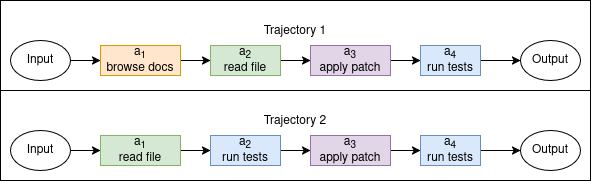
\includegraphics[width=3.2in]{../figures/action-trajectories.png}}
\caption{A visualization of an action sequence taken by an agentic system in order to solve a task.
	Each node in the graph is an action (essentially a tool call), and the edges show the sequential
	ordering of the execution.}
\label{fig-viz-seq}
\end{figure}

\subsection{Hypotheses}
For the above experiments, the following hypotheses are proposed.
\begin{enumerate}
	\item The injection of irrelevant context chunks will degrade outcome consistency
		and sequential trajectory relative to baseline runs, mimicking the reasoning shift and lost
		in the middle phenomena \cite{rodionov_reasoning_2026, liu_lost_nodate}. 
	\item Applying context pruning heuristics will yield higher sequential trajectory stability
		than a baseline which allows unbounded context accumulation.
	\item The reordering of context chunks, without altering semantic content,
		will trigger significant distributional and sequential trajectory deviations,
		because primacy and recency biases will cause different context information to lead the
		agent towards different reasoning paths \cite{liu_lost_nodate}.
\end{enumerate}

\section{Project Timeline}
The project is split up into four sequential phases:

\begin{itemize}
    \item \textbf{Phase 1 (October 2026):} set up the experiment environment by integrating
		the OpenHands agent framework~\cite{openhands_2026} and the Agent Research Environment (ARE) for
		~\cite{froger_are_2025}.
		Set up a GPU server to run open weight models (e.g. Qwen3, GPT-OSS) locally.
		Execute baseline unperturbed runs on SWE-Bench Pro~\cite{swebenchpro_2025}
		using a single-agent ReAct loop to establish reference outcome consistency and trajectory metrics.

    \item \textbf{Phase 2 (November 2026):} Run the single-agent
		experiments with context perturbations injected. Compute and analyze the metrics.

    \item \textbf{Phase 3 (December 2026):} Transition the experimental
		set-up to run a centralized multi-agent system. Inject context perturbations into individual sub-agents 
		and trace resulting error propagation across inter-agent messages.

    \item \textbf{Phase 4 (January 2027):} Aggregate quantitative reliability metrics and
		compare the results. Formulate actionable policies for context management that can
		mitigate the reliability deterioration observed during the experiments.
\end{itemize}

\bibliographystyle{IEEEtran}
\bibliography{refs}

\end{document}
